%% Copyright (c) 2015-2019, RTE (http://www.rte-france.com)
%% See AUTHORS.txt
%% All rights reserved.
%% This Source Code Form is subject to the terms of the Mozilla Public
%% License, v. 2.0. If a copy of the MPL was not distributed with this
%% file, you can obtain one at http://mozilla.org/MPL/2.0/.
%% SPDX-License-Identifier: MPL-2.0
%%
%% This file is part of Dynawo, an hybrid C++/Modelica open source time domain simulation tool for power systems.

\documentclass[a4paper, 12pt]{report}

%% Except where otherwise noted, content in this documentation is Copyright (c)
%% 2015-2019, RTE (http://www.rte-france.com) and licensed under a
%% CC-BY-4.0 (https://creativecommons.org/licenses/by/4.0/)
%% license. All rights reserved.

% Latin Modern fam­ily of fonts
\usepackage{lmodern}

\usepackage[english]{babel}

% specify encoding
\usepackage[utf8]{inputenc} % input
\usepackage[T1]{fontenc} % output
\usepackage[table]{xcolor}

% Document structure setup
\usepackage{titlesec} % To change chapter format
\setcounter{tocdepth}{3} % Add subsubsection in Content
\setcounter{secnumdepth}{3} % Add numbering for subsubsection
\setlength{\parindent}{0pt} % No paragraph indentation

% Change title format for chapter
\titleformat{\chapter}{\Huge\bf}{\thechapter}{20pt}{\Huge\bf}

% To add links on page number in Content and hide red rectangle on links
\usepackage[hidelinks, linktoc=all]{hyperref}
\usepackage[nottoc]{tocbibind}  % To add biblio in table of content
\usepackage{textcomp} % For single quote
\usepackage{url} % Allow linebreaks in \url command
\usepackage{listings} % To add code samples

% Default listings parameters
\lstset
{
  aboveskip={1\baselineskip}, % a bit of space above
  backgroundcolor=\color{shadecolor}, % choose the background color
  basicstyle={\ttfamily\footnotesize}, % use font and smaller size \small \footnotesize
  breakatwhitespace=true, % sets if automatic breaks should only happen at whitespace
  breaklines=true, % sets automatic line breaking
  columns=fixed, % nice spacing -> fixed / flexible
  mathescape=false, % escape to latex false
  numbers=left, % where to put the line-numbers
  numberstyle=\tiny\color{gray}, % the style that is used for the line-numbers
  showstringspaces=false, % do not emphasize spaces in strings
  tabsize=4, % number of spaces of a TAB
  texcl=false, % activates or deactivates LaTeX comment lines
  upquote=true % upright quotes
}

% Avoid numbering starting at each chapter for figures
\usepackage{chngcntr}
\counterwithout{figure}{chapter}

\usepackage{tikz} % macro pack­age for cre­at­ing graph­ics
\usepackage{pgfplots} % draws func­tion plots (based on pgf/tikz)

\usepackage{algorithm} % Add algorithms
\usepackage[noend]{algpseudocode} %  all end ... lines are omitted in algos

\usepackage{amsmath} % Add math­e­mat­i­cal fea­tures
\usepackage{schemabloc} % Add block diagram library (french one)

\usepackage{adjustbox} % Add box for flowchart

\usepackage{booktabs} % for toprule and midrule in tables

\usepackage{tabularx}
\usepackage{multirow}

\usepackage[nolist]{acronym} % don’t write the list of acronyms.
% Acronyms list
\begin{acronym}
\acro{BDF}{Backward Differentiation Formula}
\acro{BE}{Backward Euler}
\acro{DAE}{Differential Algebraic Equations}
\acro{IDA}{Implicit Differential-Algebraic solver}
\acro{LLNL}{Lawrence Livermore National Lab}
\acro{KINSOL}{Krylov Inexact Newton SOLver}
\acro{NR}{Newton-Raphson}
\acro{PLL}{Phase-Locked Loop}
\acro{SVC}{Static Var Compensator}
\acro{SUNDIALS}{SUite of Nonlinear and DIfferential/ALgebraic equation Solvers}
\acro{WECC}{Western Electricity Coordinating Council}
\end{acronym}

% Syntax highlight
%% Except where otherwise noted, content in this documentation is Copyright (c)
%% 2015-2019, RTE (http://www.rte-france.com) and licensed under a
%% CC-BY-4.0 (https://creativecommons.org/licenses/by/4.0/)
%% license. All rights reserved.

\usepackage{color}

\definecolor{blue}{rgb}{0,0,1}
\definecolor{lightblue}{rgb}{.3,.5,1}
\definecolor{darkblue}{rgb}{0,0,.4}
\definecolor{red}{rgb}{1,0,0}
\definecolor{darkred}{rgb}{.56,0,0}
\definecolor{pink}{rgb}{.933,0,.933}
\definecolor{purple}{rgb}{0.58,0,0.82}
\definecolor{green}{rgb}{0.133,0.545,0.133}
\definecolor{darkgreen}{rgb}{0,.4,0}
\definecolor{gray}{rgb}{.3,.3,.3}
\definecolor{darkgray}{rgb}{.2,.2,.2}
\definecolor{shadecolor}{gray}{0.925}

% **********************************************************************************
% Syntax : Bash (bash)
% **********************************************************************************

\lstdefinelanguage{bash}
{
  keywordstyle=\color{blue},
  morekeywords={
    cd,
    export,
    source},
  numbers=none,
  deletekeywords={jobs}
}

% **********************************************************************************
% Syntax : XML
% **********************************************************************************

\lstdefinelanguage{XML}
{
  morestring=[s][\color{purple}]{"}{"},
  morecomment=[s][\color{green}]{<?}{?>},
  morecomment=[s][\color{green}]{<!--}{-->},
  stringstyle=\color{black},
  identifierstyle=\color{blue},
  keywordstyle=\color{red},
  morekeywords={
    xmlns,
    xsi,
    noNamespaceSchemaLocation,
    type,
    source,
    target,
    version,
    tool,
    transRef,
    roleRef,
    objective,
    eventually}
}

% **********************************************************************************
% Syntax : Modelica (modelica)
% **********************************************************************************
\lstdefinelanguage{Modelica}{
  alsoletter={...},
  morekeywords=[1]{ % types
      Boolean,
      Integer,
      Real},
  keywordstyle=[1]\color{red},
  morekeywords=[2]{ % keywords
    algorithm,
    and,
    annotation,
    assert,
    block,
    class,
    connector,
    constant,
    discrete,
    else,
    elseif,
    elsewhen,
    end,
    equation,
    exit,
    extends,
    external,
    false,
    final,
    flow,
    for,
    function,
    if,
    in,
    inner,
    input,
    import,
    loop,
    model,
    nondiscrete,
    not,
    or,
    outer,
    output,
    package,
    parameter,
    public,
    protected,
    record,
    redeclare,
    replaceable,
    return,
    size,
    terminate,
    then,
    true,
    type,
    when,
    while},
  keywordstyle=[2]\color{darkred},
  morekeywords=[3]{ % functions
    abs,
    acos,
    asin,
    atan,
    atan2,
    Complex,
    connect,
    conj,
    cos,
    cosh,
    cross,
    der,
    edge,
    exp,
    fromPolar,
    imag,
    noEvent,
    pre,
    sign,
    sin,
    sinh,
    sqrt,
    tan,
    tanh},
  keywordstyle=[3]\color{blue},
  morecomment=[l][\color{green}]{//}, % comments
  morecomment=[s][\color{green}]{/*}{*/}, % comments
  morestring=[b][\color{pink}]{'}, % strings
  morestring=[b][\color{pink}]{"}, % strings
}


\usepackage{xspace} % Define typography
\usepackage{dirtree}
\newcommand{\Dynawo}[0]{Dyna$\omega$o\xspace}


\begin{document}

\chapter{Synchronous Machine - Infinite Bus}

The SMIB system is a well-known test case in the power system community. It is very often used to illustrate the transient or the small-signal stability of a synchronous machine. It is also used to demonstrate the behavior of a new regulation, such as a speed governor, a voltage regulation or a power-system stabilizer.

% Generic description of the non-regression test
% List of scenarios
\section{Test case description}

The following test case consists of a single machine connected to the infinite bus through two parallel lines and a transformer as presented in Figure 1.

\begin{figure}[H]
\centering
\def\factor{0.4}
\begin{tikzpicture}[every node/.style={inner sep=0,outer sep=0}]
% Infinite bus
\path (0,0)  pic[scale=0.2,local bounding box=bus] {infinite bus};
%% Transfo
\path (5,0) pic[scale=0.2,local bounding box=transfo] {transfo};
% Generator
\path (8,0) pic[scale=0.2,local bounding box=gen] {generator};
% Line 1
\draw ([yshift=0.25cm]bus.east) -- ([yshift=0.25cm]transfo.west);
% Line 1
\draw ([yshift=-0.25cm]bus.east) -- ([yshift=-0.25cm]transfo.west);
% Bus inf
\draw (bus.east) ++ (0,0.5) --++ (0,-1);
% Bus tfo 1
\draw (transfo.west) ++ (0,0.5) node (bustop) {} --++ (0,-1) node (busbottom) {};
% Bus tfo 2
\draw (transfo.east) ++ (0,0.3) node (bustop) {} --++ (0,-0.6) node (busbottom) {};
% Transfo-Generator connection
\draw (transfo.east) -- (gen.west);
\end{tikzpicture}
\caption{SMIB system representation}
\label{circuit-1}
\end{figure}

\subsection{Initial Conditions}

The infinite bus base voltage is 400 kV and the synchronous machine base voltage is 24 kV. \\

The generator is a 2220 MVA equivalent for four 555 MVA generators.\\

The lines and transformer parameters in per unit on 100 MVA base are:
\begin{center}
\begin{tabular}{l|l|l}
   $R_1=0$ & $R_2=0$ & $R_{Tfo}=0$ \\
   $X_1=0.022522$ & $X_2=0.04189$ & $X_{Tfo}=0.00675$ \\
\end{tabular}
\end{center}

The reference angle for the load flow is set at the infinite bus, and the voltage amplitude at the machine terminal is set to 1. \\

The load flow results in per unit on 100 MVA base are:
\begin{center}
\begin{tabular}{l|l|l}
   $U_{Inf}=0.90081$ & $U_{SM}=1$ & $P_{SM}=19.98$ \\
   $\Theta_{Inf}=0rad$ & $\Theta_{SM}=0.49445rad$ & $Q_{SM}=9.68$ \\
\end{tabular}
\end{center}

\subsection{Models}

The equivalent generator parameters are given in per unit on 2220 MVA - 24 kV (no transformer included, no saturation):
\begin{center}
\begin{tabular}{l|l|l|l}
   $R_a=0.003$ & $X_l=0.15$ & $H=3.5$ & $D=0$ \\
   $X_d=1.81$ & $T'_d0=8s$ & $X_q=1.76$ & $T'_q0=1s$ \\
   $X'_d=0.30$ & $T''_d0=0.03s$ & $X'_q=0.65$ & $T''_q0=0.07s$ \\
   $X''_d=0.23$ & & $X''_q=0.25$ &  \\
\end{tabular}
\end{center}

The system reference frequency omegaRef is set to 1.\\
The machine is controlled by a proportional speed governor and a proportional voltage regulator. \\

The voltage regulator is as follows:
\begin{figure}[H]
\centering
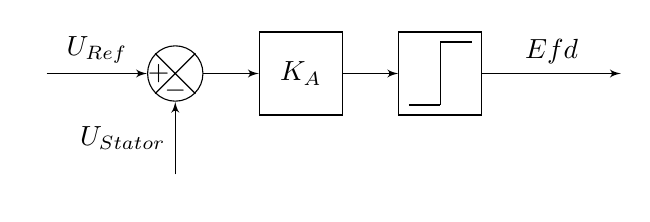
\begin{tikzpicture}
\sbEntree{E}
\sbCompSum[5]{errAVR}{E}{}{-}{+}{}
\sbRelier[$U_{Ref}$]{E}{errAVR}
\sbDecaleNoeudy[4]{errAVR}{Us}
\sbRelier[$U_{Stator}$]{Us}{errAVR}
\sbBloc{Gain}{$K_A$}{errAVR}
\sbRelier{errAVR}{Gain}
\sbBlocL{Limiter}{\tikz {\draw (-0.4,-0.4) -- (0,-0.4);\draw (0,-0.4) -- (0,0.4); \draw (0,0.4) -- (0.4,0.4); }}{Gain}
\sbSortie[5]{S}{Limiter}
\sbRelier[$Efd$]{Limiter}{S}
\end{tikzpicture}
\caption{Voltage regulator}
\end{figure}

The speed governor is as follows:
\begin{figure}[H]
\centering
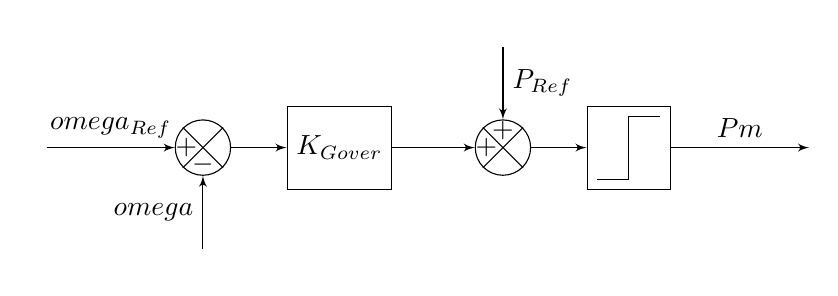
\begin{tikzpicture}
\sbEntree{E}
\sbCompSum[6]{errW}{E}{}{-}{+}{}
\sbRelier[$omega_{Ref}$]{E}{errW}
\sbDecaleNoeudy[4]{errW}{Omega}
\sbRelier[$omega$]{Omega}{errW}
\sbBloc{Gain}{$K_{Gover}$}{errW}
\sbRelier{errW}{Gain}
\sbCompSum{sumP}{Gain}{+}{}{+}{}
\sbRelier{Gain}{sumP}
\sbDecaleNoeudy[-4]{sumP}{PRef}
\sbRelier[$P_{Ref}$]{PRef}{sumP}
\sbBlocL{Limiter}{\tikz {\draw (-0.4,-0.4) -- (0,-0.4);\draw (0,-0.4) -- (0,0.4); \draw (0,0.4) -- (0.4,0.4); }}{sumP}
\sbSortie[5]{S}{Limiter}
\sbRelier[$Pm$]{Limiter}{S}
\end{tikzpicture}
\caption{Speed Governor}
\end{figure}

The voltage regulator parameters are:
\begin{center}
\begin{tabular}{l|l}
   $K_A=20$ & $Efd_{Max}=5$  \\
    & $Efd_{Min}=-5$   \\
\end{tabular}
\end{center}

The speed governor parameters are:
\begin{center}
\begin{tabular}{l|l}
   $P_{Nom}=2200$ & $P_{Max}=2200$  \\
   $K_{Gover}=5$ & $P_{Min}=0$   \\
\end{tabular}
\end{center}

\subsection{Scenarios}
The simulated scenarios are :
\begin{itemize}
\item a step on the mechanical power;
\item a step on the excitation voltage;
\item a reactive load variation;
\item a disconnection of line 2;
\item a three-phase fault at the transformer high level terminal;
\end{itemize}

\subsection{Solver}
The solver used is the variable time step solver IDA with the following parameters:
\begin{itemize}
\item $Order$=2;
\item $Accuracy_{Rel}$=10e-6;
\item $Accuracy_{Abs}$=10e-6;
\end{itemize}

\newpage
\section{Results}

\subsection{Step on the mechanical power}

At $t=1s$, the reference mechanical power $P_{Ref}$ is increased by 0.02 pu\\

We observe that the active power is increased by 0.02 pu The voltage drop between the infinite bus and the machine terminal is consequently increased, resulting in a slight decrease of the machine terminal voltage.\\

\begin{figure}[H]
\subfigure[Generator stator voltage (kV)]
{%
  \begin{tikzpicture}
    \begin{axis}[height = 2.4in]
        \addplot[color=blue!50]
        table[x=time, y expr=\thisrow{SM_generator_UPu}*24]
        {../SMIB_1_StepPm/reference/outputs/curves/curves.csv};
    \end{axis}
  \end{tikzpicture}
}
\subfigure[Generator active power (pu)]
{%
  \begin{tikzpicture}
    \begin{axis}[height = 2.4in]
        \addplot[color=blue!50]
        table[x=time, y expr=\thisrow{SM_generator_PGenPu}*100/2220]
        {../SMIB_1_StepPm/reference/outputs/curves/curves.csv};
    \end{axis}
  \end{tikzpicture}
}
\caption{Step on the mechanical power}
\end{figure}

\newpage
\subsection{Step on the excitation voltage}

At $t=1s$, the reference voltage of the voltage regulation $U_{Ref}$ is decreased by 0.1 pu\\

We observe that the reactive power injected by the machine is decreased in order to decrease the machine terminal voltage.\\

\begin{figure}[H]
\subfigure[Generator stator voltage (kV)]
{%
  \begin{tikzpicture}
    \begin{axis}[height = 2.4in]
        \addplot[color=blue!50]
        table[x=time, y expr=\thisrow{SM_generator_UPu}*24]
        {../SMIB_2_StepEfd/reference/outputs/curves/curves.csv};
    \end{axis}
  \end{tikzpicture}
}
\subfigure[Generator reactive power (pu)]
{%
  \begin{tikzpicture}
    \begin{axis}[height = 2.4in]
        \addplot[color=blue!50]
        table[x=time, y expr=\thisrow{SM_generator_QGenPu}*100/2220]
        {../SMIB_2_StepEfd/reference/outputs/curves/curves.csv};
    \end{axis}
  \end{tikzpicture}
}
\caption{Step on the excitation voltage}
\end{figure}

\newpage
\subsection{Load Variation}

At $t=1s$, we apply a reactive load change at the machine terminal of 0.5 pu\\

We observe that the voltage drops directly after the load modification. In order to counter this voltage drop, the voltage regulation acts and the machine starts injecting more reactive power. As a consequence, the voltage is increased again but stabilizes at a value lower than the initial one. \\

\begin{figure}[H]
\subfigure[Generator stator voltage (kV)]
{%
  \begin{tikzpicture}
    \begin{axis}[height = 2.4in]
        \addplot[color=blue!50]
        table[x=time, y expr=\thisrow{SM_generator_UPu}*24]
        {../SMIB_3_LoadVarQ/reference/outputs/curves/curves.csv};
    \end{axis}
  \end{tikzpicture}
}
\subfigure[Generator reactive power (pu)]
{%
  \begin{tikzpicture}
    \begin{axis}[height = 2.4in]
        \addplot[color=blue!50]
        table[x=time, y expr=\thisrow{SM_generator_QGenPu}*100/2220]
        {../SMIB_3_LoadVarQ/reference/outputs/curves/curves.csv};
    \end{axis}
  \end{tikzpicture}
}
\caption{Load variation}
\end{figure}

\newpage
\subsection{Line Opening}

At $t=1s$, we open one of the two lines of the system.\\

We observe that the system is oscillating after the event but stabilizes after a few seconds. The active power is restored to its pre-event value but the reactive power is changed in response to the terminal voltage change (action of the voltage regulation). \\

\begin{figure}[H]
\subfigure[Generator stator voltage (kV)]
{%
  \begin{tikzpicture}
    \begin{axis}[height = 1.7in]
        \addplot[color=blue!50]
        table[x=time, y expr=\thisrow{SM_generator_UPu}*24]
        {../SMIB_4_DisconnectLine/reference/outputs/curves/curves.csv};
    \end{axis}
  \end{tikzpicture}
}
\subfigure[Generator active power (pu)]
{%
  \begin{tikzpicture}
    \begin{axis}[height = 1.7in]
        \addplot[color=blue!50]
        table[x=time, y expr=\thisrow{SM_generator_PGenPu}*100/2220]
        {../SMIB_4_DisconnectLine/reference/outputs/curves/curves.csv};
    \end{axis}
  \end{tikzpicture}
}
\subfigure[Generator reactive power (pu)]
{%
  \begin{tikzpicture}
    \begin{axis}[height = 1.7in]
        \addplot[color=blue!50]
        table[x=time, y expr=\thisrow{SM_generator_QGenPu}*100/2220]
        {../SMIB_4_DisconnectLine/reference/outputs/curves/curves.csv};
    \end{axis}
  \end{tikzpicture}
}
\caption{Line opening}
\end{figure}

\newpage
\subsection{Three-Phase Fault}

At $t=1s$, a 0.07s three-phase fault is applied at the transformer high voltage terminal.\\

We observe that active power during the fault is zero and that it is restored to its pre-event value after fault clearance. During the fault the machine terminal voltage drops but there is a remaning voltage at the node. The machine naturally injects reactive power during the fault. \\

\begin{figure}[H]
\subfigure[Generator stator voltage (kV)]
{%
  \begin{tikzpicture}
    \begin{axis}[height = 1.7in]
        \addplot[color=blue!50]
        table[x=time, y expr=\thisrow{SM_generator_UPu}*24]
        {../SMIB_5_Fault/reference/outputs/curves/curves.csv};
    \end{axis}
  \end{tikzpicture}
}
\subfigure[Generator active power (pu)]
{%
  \begin{tikzpicture}
    \begin{axis}[height = 1.7in]
        \addplot[color=blue!50]
        table[x=time, y expr=\thisrow{SM_generator_PGenPu}*100/2220]
        {../SMIB_5_Fault/reference/outputs/curves/curves.csv};
    \end{axis}
  \end{tikzpicture}
}
\subfigure[Generator reactive power (pu)]
{%
  \begin{tikzpicture}
    \begin{axis}[height = 1.7in]
        \addplot[color=blue!50]
        table[x=time, y expr=\thisrow{SM_generator_QGenPu}*100/2220]
        {../SMIB_5_Fault/reference/outputs/curves/curves.csv};
    \end{axis}
  \end{tikzpicture}
}
\caption{Three-phase fault}
\end{figure}


\end{document}
